\documentclass[acmsmall,screen,nonacm]{acmart}
\usepackage[greek,english]{babel}
\usepackage{float}
\usepackage{alphabeta} 
\usepackage{amsmath}
\usepackage{booktabs}
\usepackage{listings}
\usepackage{url}
\usepackage{graphicx}

\babelfont[greek]{rm}{Noto Serif}
\babelfont[greek]{sf}{Noto Sans}
\sloppy

\title{Smart Waste Bin}
\subtitle{Ολοκληρωμένο Σύστημα IoT για την Έξυπνη Διαχείριση Απορριμμάτων \\ Προηγμένες Τεχνικές Προγραμματισμού (CK801)}

\author{\NoCaseChange{Αθανάσιος Μήτσης 1100944\& Βασίλειος Ρούσσης 1104685\& Δημήτριος Φιλόπουλος 1101130}}
\affiliation{
	\institution{\newline Τμήμα ΗΜ\&ΤΥ, Πανεπιστήμιο Πατρών}
	\country{Ελλάδα}
}
\captionsetup[table]{position=bottom}

\renewcommand{\shortauthors}{Α.Μ, Β.Ρ, Δ.Φ.}

\begin{document}
	
	\maketitle
	
	\section{Εισαγωγή}
	
	Στην παρούσα εργασία παρουσιάζεται η σχεδίαση, υλοποίηση και αξιολόγηση ενός ολοκληρωμένου, κατανεμημένου συστήματος IoT για τη μετατροπή ενός κοινού κάδου απορριμμάτων σε έξυπνη, αυτοματοποιημένη συσκευή. Το σύστημα βασίζεται σε ένα Raspberry Pi εξοπλισμένο με αισθητήρα κίνησης PIR (HC-SR501) για την ανίχνευση ρίψης απορριμμάτων. Τα δεδομένα που λαμβάνονται από τον αισθητήρα διοχετεύονται μέσω του πρωτοκόλλου MQTT. 

	Η μοντελοποίηση των δεδομένων πραγματοποιείται με χρήση σημασιολογικού ιστού (JSON-LD) βασισμένου στα πρότυπα SOSA και SAREF. Παράλληλα, αναπτύχθηκε μια διεπαφή REST API με Flask-RESTx για τη σύγχρονη προσπέλαση των δεδομένων, ενώ υλοποιήθηκαν τρείς εικονικοί αισθητήρες (virtual sensors): ένας βασισμένος σε ντετερμινιστικούς κανόνες για τον υπολογισμό της έντασης χρήσης, ένας βασισμένος σε μηχανική μάθηση για την πρόβλεψη μελλοντικής δραστηριότητας, και ένας όπου προσωμοιώνει 4 αισθητήρες, εναν υπερηχητικό αισθητήρα, έναν αισθητήρα βάρους, έναν αισθητήρα θερμοκρασίας και έναν μετρητή ποσοστού μπαταρίας. Τέλος, το σύστημα ενσωματώνει τη low-code πλατφόρμα Node-RED για την σχεδίαση ροών, την αποστολή ειδοποιήσεων κρίσιμης κατάστασης και την οπτικοποίηση των δεδομένων σε ένα Dashboard στο Home Assistant.

	\section{Υλοποίηση σταδίων για την εκπόνηση της εργασίας}

	Το σύστημα υλοποιεί έναν πλήρη αγωγό επεξεργασίας δεδομένων, ξεκινώντας από το χαμηλό επίπεδο της διεπαφής με το υλικό και φτάνοντας έως το υψηλό επίπεδο των σημασιολογικών δεδομένων, των RESTful υπηρεσιών, των αλγορίθμων πρόβλεψης και των low-code διεπαφών χρήστη. Η ανάπτυξη οργανώθηκε σε 10 διακριτά ορόσημα (Milestones), τα οποία κάλυψαν όλο το φάσμα της σύγχρονης μηχανικής λογισμικού για συστήματα IoT: από τη διαχείριση νημάτων και των παράλληλων ουρών, την κοντεϊνεροποίηση (containerization) μέσω Docker, έως τη σημασιολογική μοντελοποίηση, το πρωτόκολλο MQTT, τον σχεδιασμό ενός UI/Dashboard με τη χρήση του Home Assistant, την εκπαίδευση μοντέλων Random Forest και την οπτικοποίηση ροών σε Node-RED.
	
	\section{Αρχιτεκτονική και Τοπολογία Συστήματος}
	Για την εξασφάλιση της επεκτασιμότητας και της ανεξαρτησίας των επιμέρους στοιχείων, το σύστημα σχεδιάστηκε με βάση μια \textbf{κατανεμημένη αρχιτεκτονική δημοσίευσης/εγγραφής (Publish/Subscribe)} με τη χρήση του πρωτοκόλλου MQTT. Η διαχείριση και η εκτέλεση των υπηρεσιών πραγματοποιείται μέσω της πλατφόρμας Docker Compose, επιτρέποντας την απομόνωση των διεργασιών και την εύκολη μεταφερσιμότητα σε οποιαδήποτε embedded ή edge συσκευή.
	
	\begin{figure}[H]
		\centering
		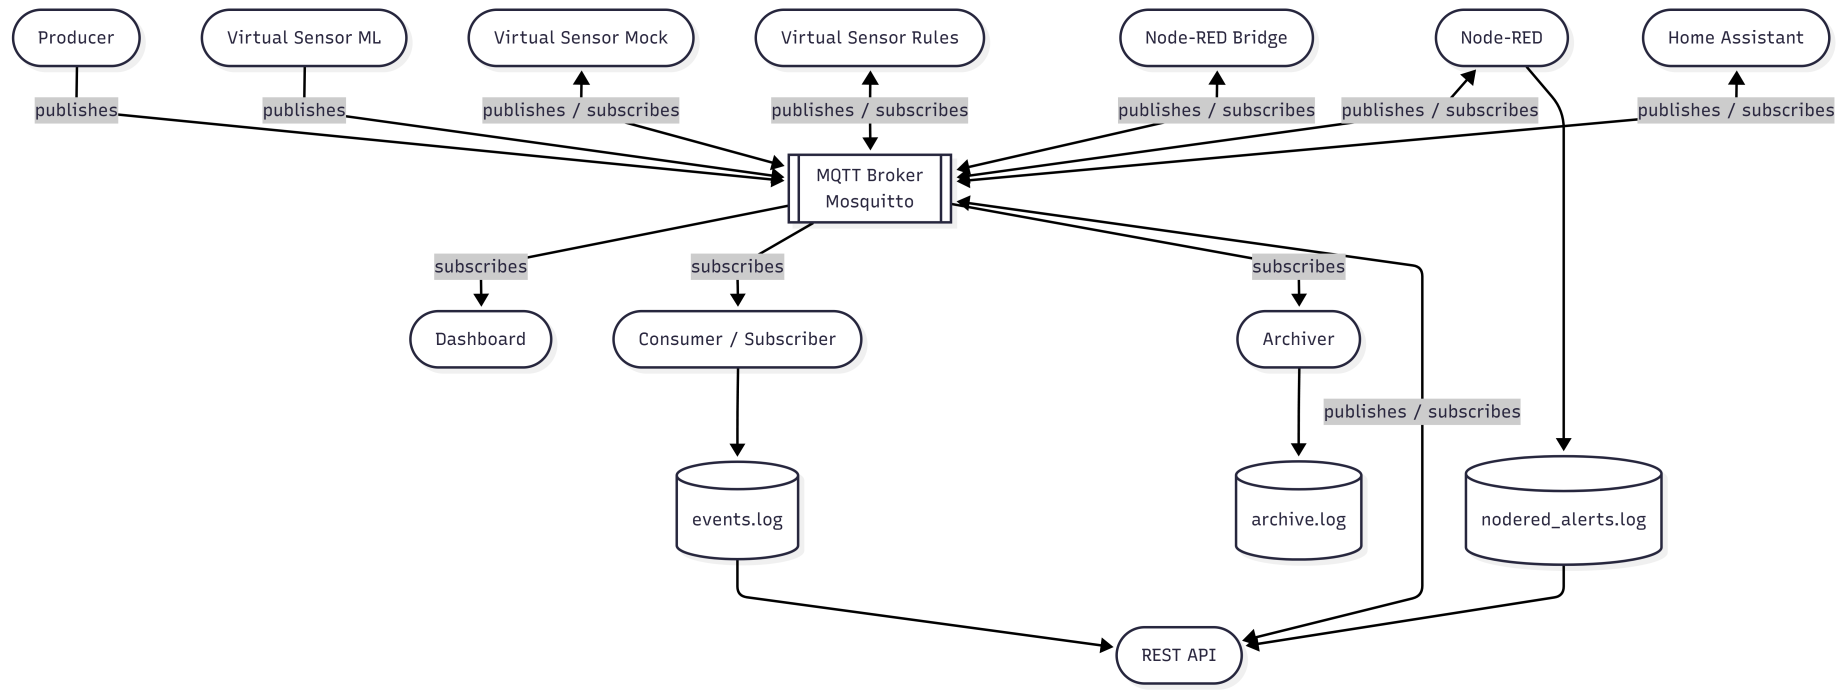
\includegraphics[width=0.85\textwidth]{architecture.png}
		\caption{Αρχιτεκτονική και Τοπολογία του Συστήματος IoT (Docker \& MQTT Message Broker)}
		\label{fig:architecture}
	\end{figure}
	
	\subsection{Ανάλυση Υπηρεσιών Docker}
	Η τοπολογία του συστήματος αποτελείται από τις εξής βασικές υπηρεσίες, όπως ορίζονται στο αρχείο \texttt{docker-compose.yml}:
	
	\begin{enumerate}
		\item \textbf{Broker:} Χρησιμοποιεί το \texttt{eclipse-mosquitto:latest} ως το κεντρικό  σύστημα διανομής μηνυμάτων.
		\item \textbf{Producer:} Συνδέεται απευθείας με τις θύρες GPIO του Raspberry Pi, λαμβάνει τις μετρήσεις του αισθητήρα, τις φιλτράρει και τις δημοσιεύει στο broker, μαζί με την κατάσταση και τον αριθμό χρήσεων του κάδου.
		\item \textbf{Consumer:} Εγγράφεται στα κατάλληλα topics και καταγράφει τα γεγονότα σε μορφή JSONL στο αρχείο \texttt{motion\_events.log}.
		\item \textbf{Dashboard:} Είναι ένα βασικό dashboard που προβάλλεται από το terminal με JSON Objects, για να παρατηρούμε τη χρήση του κάδου και για να μπορούμε να κάνουμε διορθώσεις in-real-time.
		\item \textbf{Archiver :} Αναλαμβάνει τη μόνιμη αρχειοθέτηση όλων των μηνυμάτων της τοπολογίας \texttt{smartbin/\#} στο αρχείο \texttt{archive.log}.
		\item \textbf{REST API:} Μια Flask εφαρμογή που εκθέτει REST endpoints για τη σύγχρονη άντληση της κατάστασης του συστήματος και των αισθητήρων.
		\item \textbf{Virtual Sensor Rules \& ML:} Δύο ανεξάρτητες υπηρεσίες που επεξεργάζονται τα πρωτογενή γεγονότα κίνησης και παράγουν υψηλότερου επιπέδου πληροφορία (ένταση χρήσης και προβλέψεις).
		\item \textbf{Home Assistant \& Node-RED:} Οι πλατφόρμες οπτικοποίησης, ελέγχου και low-code αυτοματισμών.
		\item \textbf{Node-RED Bridge:} Υλοποιεί την αμφίδρομη επικοινωνία μεταξύ του Node-RED και του κεντρικού συστήματος. Διαχειρίζεται την καταγραφή των \emph{alerts} στο \texttt{nodered\_alerts.log}, την επεξεργασία των \emph{acknowledgements} (\emph{ack}) και των \emph{solved states}.
		\item \textbf{Virtual Sensor Generic Data:} Εγγράφεται στα \emph{topics} των προσομοιωμένων αισθητήρων (ultrasonic, temperature, weight, battery), εξάγει τις τιμές τηλεμετρίας τους και τις δημοσιεύει σε \emph{simplified state topics}. Παράλληλα, αναλαμβάνει το \emph{MQTT Discovery} του Home Assistant, στέλνοντας \emph{discovery config payloads}.
	\end{enumerate}
	
	\section{Ενσωμάτωση Αισθητήρα και Φιλτράρισμα Ψηφιακού Σήματος}
	Το σύστημα περιέχει έναν αισθητήρα κίνησης υπερύθρων \textbf{HC-SR501 PIR}, ο οποίος συνδέεται στο Raspberry Pi. Η ανάγνωση και επεξεργασία του σήματος υλοποιείται μέσω της βιβλιοθήκης \texttt{pirlib}.
	
	\subsection{Noise Filtering \& Debouncing}
	Οι αισθητήρες PIR παρουσιάζουν συχνά ηλεκτρικό θόρυβο ή στιγμιαίες ψευδείς μεταβολές σήματος. Για την αποφυγή λανθασμένων καταγραφών, ο \texttt{PirInterpreter} εφαρμόζει δύο διαδοχικά ψηφιακά φίλτρα:
	
	\begin{enumerate}
		\item \textbf{Ελάχιστος Χρόνος Ενεργοποίησης:} Το ψηφιακό σήμα εισόδου πρέπει να παραμείνει σε κατάσταση HIGH ($V_{out} \approx 3.3\text{V}$) συνεχόμενα για ένα ελάχιστο χρονικό διάστημα $T_{high}$ (π.χ. $T_{high} = 0.5$ δευτερόλεπτα) προκειμένου να θεωρηθεί ως έγκυρο γεγονός κίνησης:
		\begin{equation}
			\Delta t_{high} \ge T_{high}
		\end{equation}
		\item \textbf{Cooldown Period:} Μετά την επιτυχή ανίχνευση ενός γεγονότος, επιβάλλεται μια περίοδος αποχής $T_{cool}$ (π.χ. $T_{cool} = 5.0$ δευτερόλεπτα) κατά την οποία οποιαδήποτε νέα ενεργοποίηση αγνοείται. Αυτό αποτρέπει την πολλαπλή καταγραφή ενός και μόνο γεγονότος ρίψης απορριμμάτων:
		\begin{equation}
			t_{event, k} - t_{event, k-1} > T_{cool}
		\end{equation}
	\end{enumerate}
	
	\section{Σημασιολογική Μοντελοποίηση και MQTT Τοπολογία}
	Για να καταστούν τα δεδομένα του συστήματος αυτο-περιγραφόμενα και διαλειτουργικά, εφαρμόστηκαν τεχνολογίες Semantic Web. 
	
	\subsection{Μοντελοποίηση JSON-LD}
	Κάθε γεγονός κίνησης που παράγεται από τον \texttt{Producer} περιλαμβάνει ενσωματωμένο πλαίσιο \texttt{@context} και τύπο \texttt{@type}, συνδέοντας τα δεδομένα με διεθνώς αναγνωρισμένες οντολογίες:
	\begin{itemize}
		\item \textbf{SOSA (Sensor, Observation, Sample, and Actuation):} Χρησιμοποιείται για την αναπαράσταση των παρατηρήσεων (\texttt{sosa:Observation}) και του αισθητήρα (\texttt{sosa:Sensor}).
		\item \textbf{SAREF (Smart Applications REference Ontology):} Μοντελοποιεί τον ίδιο τον κάδο ως έξυπνη συσκευή (\texttt{saref:Appliance}).
		\item \textbf{BOT (Building Topology Ontology):} Περιγράφει το φυσικό περιβάλλον εγκατάστασης (\texttt{bot:Space}).
	\end{itemize}
	
	\begin{figure}[H]
		\centering
		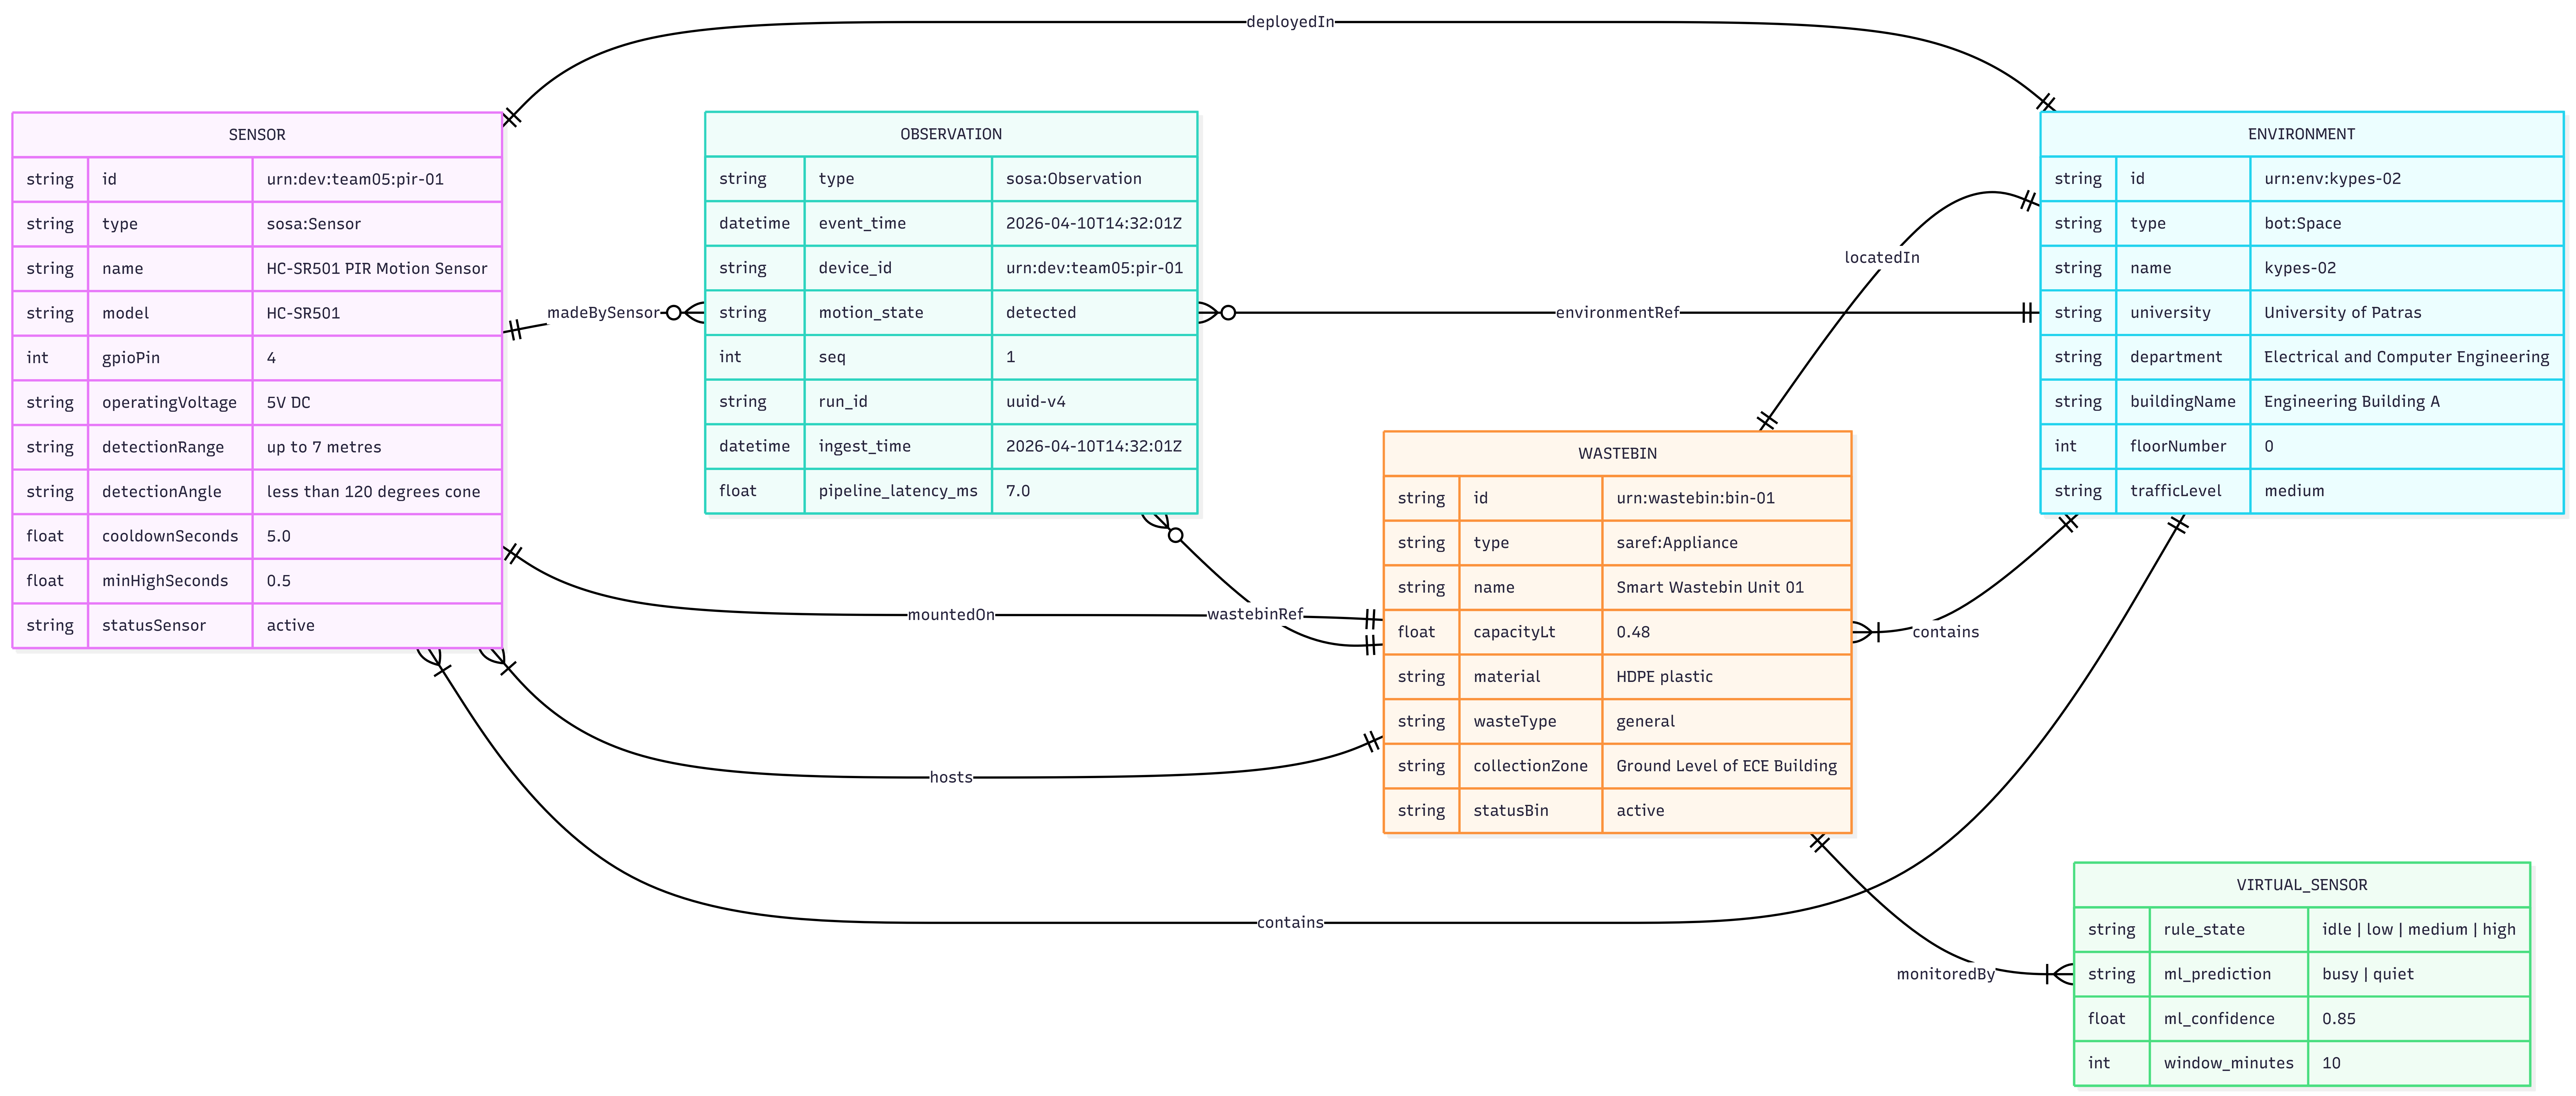
\includegraphics[width=0.85\textwidth]{jsonld_schema.png}
		\caption{Σημασιολογική Μοντελοποίηση και Διάγραμμα Οντολογιών JSON-LD (SOSA, SAREF, BOT)}
		\label{fig:jsonld_schema}
	\end{figure}
	
	Τα γεγονότα εμπλουτίζονται με μοναδικούς αναγνωριστικούς κωδικούς URN (π.χ. \texttt{urn:dev:team05:pir-01} για τον αισθητήρα, \texttt{urn:wastebin:bin-01} για τον κάδο και \texttt{urn:env:kypes-02} για το δωμάτιο) και περιλαμβάνουν μετρικές όπως το χρόνο παραγωγής (\texttt{event\_time}), το χρόνο λήψης (\texttt{ingest\_time}) και την καθυστέρηση (\texttt{pipeline\_latency\_ms}).
	
	\subsection{MQTT Topic Hierarchy}
	Ορίστηκε μια αυστηρή και ιεραρχικά δομημένη τοπολογία θεμάτων για τη διευκόλυνση της δρομολόγησης, του φιλτραρίσματος των μηνυμάτων και της απρόσκοπτης ενσωμάτωσης των επιμέρους υπηρεσιών. Τα σημαντικότερα θέματα της τοπολογίας ταξινομούνται στις εξής κατηγορίες:

	\subsubsection{1. Sensor Telemetry \& Events}
	\begin{itemize}
		\item \texttt{smartbin/+/+/events}: Δημοσίευση των σημασιολογικών JSON-LD γεγονότων (π.χ. \texttt{smartbin/bin-01/pir-01/events}). Περιλαμβάνει επιπλέον:
		\begin{itemize}
			\item \texttt{smartbin/bin-01/ultrasonic-01/events}: Γεγονότα επιπέδου πληρότητας (ποσοστό \% και απόσταση).
			\item \texttt{smartbin/bin-01/weight-01/events}: Γεγονότα βάρους απορριμμάτων.
		\end{itemize}
		\item \texttt{smartbin/+/+/motion}: Απλό σήμα κατάστασης (\texttt{detected}/\texttt{clear}) για άμεση ενσωμάτωση στο Home Assistant.
		\item \texttt{smartbin/+/+/event\_count}: Συνολικός αριθμός ανιχνεύσεων κίνησης (μετρητής) για την παρακολούθηση της δραστηριότητας.
	\end{itemize}
	
	\subsubsection{2.Device Status \& Diagnostics}
	\begin{itemize}
		\item \texttt{smartbin/+/status}: Κατάσταση σύνδεσης του κάδου (\texttt{active}/\texttt{offline}) με χρήση της λειτουργίας \emph{Last Will and Testament (LWT)} του MQTT.
		\item \texttt{smartbin/nodered/heartbeat}: Μήνυμα ελέγχου ενεργής σύνδεσης (heartbeat) για τη διάγνωση της υγείας της low-code πλατφόρμας Node-RED.
	\end{itemize}

	\subsubsection{3. Virtual Sensors \& Edge AI}
	\begin{itemize}
		\item \texttt{smartbin/+/usage\_intensity}: Δημοσίευση της έντασης χρήσης (\texttt{idle}, \texttt{low}, \texttt{medium}, \texttt{high}) όπως υπολογίζεται από τον κανόνα του εικονικού αισθητήρα.
		\item \texttt{smartbin/+/usage\_prediction}: Δημοσίευση της πρόβλεψης του ML μοντέλου (\texttt{busy}/\texttt{quiet}) μαζί με το βαθμό εμπιστοσύνης (confidence score).
	\end{itemize}

	\subsubsection{4. Σύστημα Ειδοποιήσεων και Διαχείρισης Συμβάντων }
	\begin{itemize}
		\item \texttt{smartbin/+/alerts/current\_status}: Η τρέχουσα κατάσταση της ειδοποίησης (π.χ. \texttt{active}, \texttt{idle}, \texttt{acknowledged}, \texttt{solved}) με επιπρόσθετα attributes τηλεμετρίας.
		\item \texttt{smartbin/+/alerts/ack}: Επιβεβαίωση (acknowledgement) της ειδοποίησης από τον χειριστή.
		\item \texttt{smartbin/+/alerts/solved}: Σήμανση οριστικής επίλυσης της ειδοποίησης.
	\end{itemize}

	\subsubsection{5. Έλεγχος και Node-RED Integration}
	\begin{itemize}
		\item \texttt{smartbin/nodered/alert\_log}: Καταγραφή ιστορικών ειδοποιήσεων από το Node-RED.
		\item \texttt{smartbin/nodered/alert\_ack}: Λήψη εντολής επιβεβαίωσης ειδοποίησης από το Home Assistant / Dashboard.
		\item \texttt{smartbin/nodered/alert\_solved}: Λήψη εντολής επίλυσης ειδοποίησης από το Home Assistant / Dashboard.
	\end{itemize}
	
	\section{Flask REST API και Formal Specifications}
	Η εφαρμογή REST API (\texttt{src/api.py}) αναπτύχθηκε με χρήση του framework \textbf{Flask-RESTx}. Παρέχει μια πλήρη Swagger διεπαφή που επιτρέπει τη σύγχρονη ανάγνωση της κατάστασης των κάδων, των αισθητήρων και των ιστορικών γεγονότων. 
	
	Επιπλέον, το API λειτουργεί ως αμφίδρομη γέφυρα με το MQTT, προσφέροντας endpoint (\texttt{/mqtt/publish}) για τη δημοσίευση μηνυμάτων στο broker μέσω HTTP POST, καθώς και endpoints για την ανάγνωση των τελευταίων καταγεγραμμένων τιμών κάθε θέματος. Η αρχιτεκτονική του συστήματος τεκμηριώνεται πλήρως μέσω δύο τυποποιημένων προδιαγραφών:
	\begin{itemize}
		\item \textbf{OpenAPI Specification (Swagger):} Για την περιγραφή της σύγχρονης pull-based HTTP διεπαφής.
		\item \textbf{AsyncAPI Specification:} Για την επίσημη τεκμηρίωση της push-based MQTT αρχιτεκτονικής, των θεμάτων και των σχημάτων (schemas) των μηνυμάτων.
	\end{itemize}
	
	\begin{figure}[H]
		\centering
		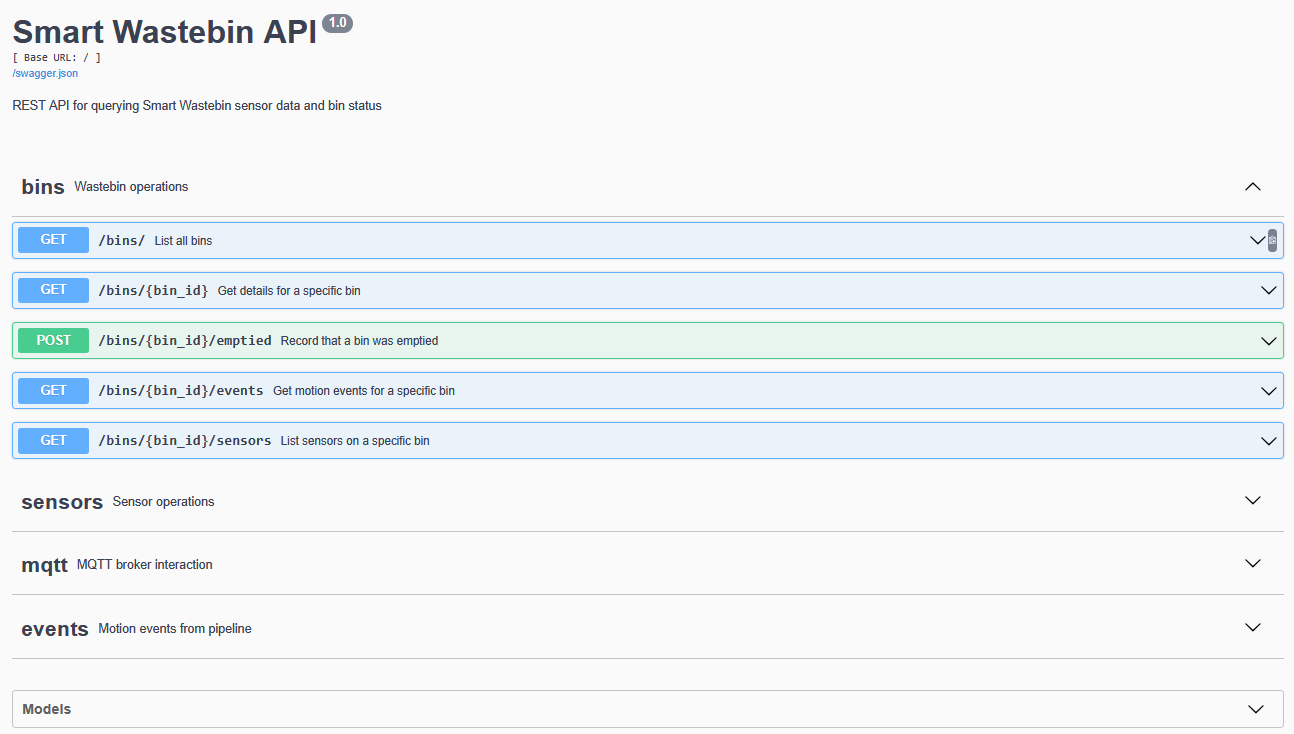
\includegraphics[width=0.85\textwidth]{swagger_ui.png}
		\caption{Διεπαφή Swagger UI του Flask REST API}
		\label{fig:swagger_ui}
	\end{figure}
	
	\begin{figure}[H]
		\centering
		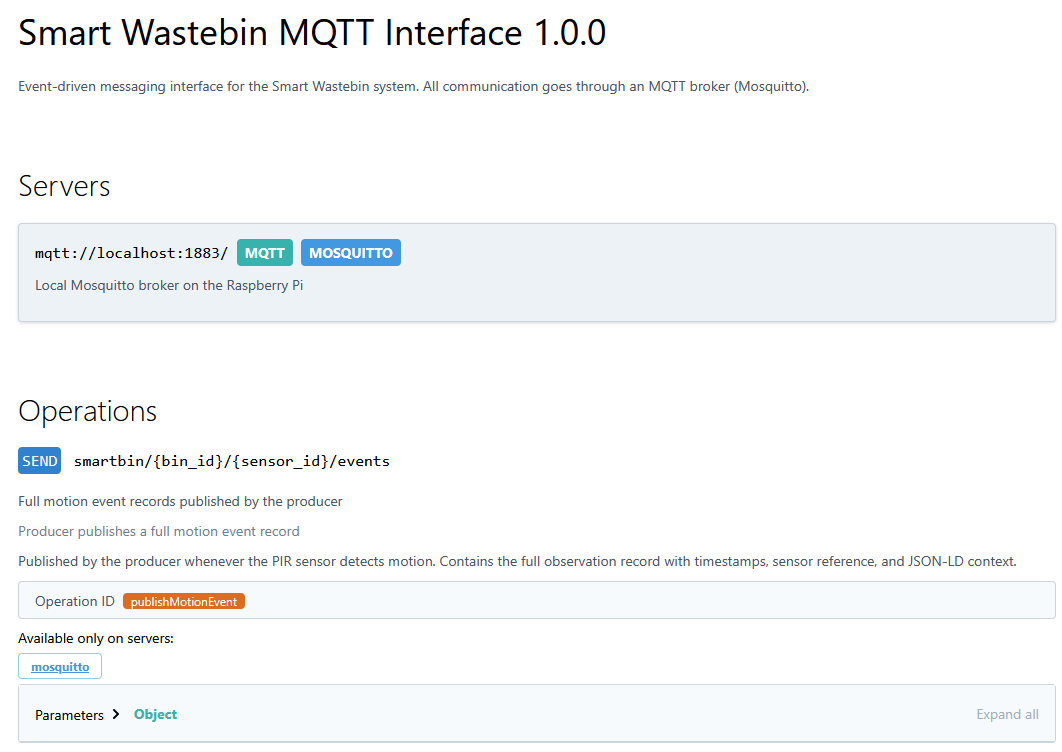
\includegraphics[width=0.85\textwidth]{asyncapi.png}
		\caption{Τεκμηρίωση της Event-Driven Αρχιτεκτονικής μέσω AsyncAPI}
		\label{fig:asyncapi}
	\end{figure}
	
	\section{Εικονικοί Αισθητήρες (Virtual Sensors)}
	Ένα από τα πιο προηγμένα χαρακτηριστικά του συστήματος είναι η υλοποίηση Virtual Sensors, οι οποίοι συνδυάζουν πρωτογενείς μετρήσεις για την παραγωγή πληροφορίας υψηλότερης προστιθέμενης αξίας.
	
	\subsection{Virtual Sensor βασισμένος σε Κανόνες (Rule-based)}
	Η υπηρεσία \texttt{virtual\_sensor\_rules.py} υπολογίζει την ένταση χρήσης του κάδου σε πραγματικό χρόνο. Διατηρεί ένα sliding window διάρκειας $Χ$ λεπτών (π.χ. $Χ = 10$) και μετράει το πλήθος των γεγονότων κίνησης $E_{count}$. Το Usage State καθορίζεται από τις εξής συνθήκες:
	\begin{equation}
		\text{Usage State} = \begin{cases}
			\text{idle}, & E_{count} = 0 \\
			\text{low}, & 0 < E_{count} \le 5 \\
			\text{medium}, & 5 < E_{count} \le 15 \\
			\text{high}, & E_{count} > 15
		\end{cases}
	\end{equation}
	
	\subsection{Virtual Sensor βασισμένος σε Μηχανική Μάθηση (ML-based)}
	Η υπηρεσία \texttt{virtual\_sensor\_ml.py} πραγματοποιεί προβλέψεις για το αν ο κάδος θα είναι πολυάσχολος (\texttt{busy}) ή ήσυχος (\texttt{quiet}) κατά την επόμενη ώρα. 
	
	Χρησιμοποιεί ένα μοντέλο \textbf{Random Forest Classifier} (50 estimators), το οποίο εκπαιδεύτηκε (\texttt{train\_model.py}) σε συνθετικά δεδομένα 30 ημερών που προσομοιώνουν ρυθμούς χρήσης ανάλογα με την ώρα και την ημέρα (π.χ. αυξημένη κίνηση τις καθημερινές κατά τις ώρες 11:00-14:00). Το διάνυσμα χαρακτηριστικών εισόδου $\vec{x}$ ορίζεται ως:
	\begin{equation}
		\vec{x} = \begin{bmatrix}
			D_{week} \\
			H_{next} \\
			I_{weekend}
		\end{bmatrix}
	\end{equation}
	όπου $D_{week} \in \{0,\dots,6\}$ είναι η ημέρα της εβδομάδας, $H_{next} \in \{0,\dots,23\}$ είναι η επόμενη ώρα και $I_{weekend} \in \{0, 1\}$ είναι δείκτης σαββατοκύριακου. Το μοντέλο επιστρέφει την κλάση πρόβλεψης και το βαθμό εμπιστοσύνης (confidence score) βάσει των πιθανοτήτων της Random Forest:
	\begin{equation}
		\hat{y} = \arg\max_{c} P(y = c \mid \vec{x})
	\end{equation}
	
	\textbf{Σημείωση Υλοποίησης:} Επειδή το εκπαιδευμένο μοντέλο δεν αποθηκεύεται απευθείας στον πηγαίο κώδικα, αποτελεί προαπαιτούμενο βήμα η εκτέλεση του σεναρίου \texttt{train\_model.py} για την παραγωγή του αρχείου \texttt{busy\_predictor.joblib}. Μόνο μετά τη δημιουργία του αρχείου αυτού μπορεί να εκκινηθεί επιτυχώς η υπηρεσία \texttt{virtual\_sensor\_ml.py} μέσω του Docker Compose.
	
	\begin{figure}[H]
		\centering
		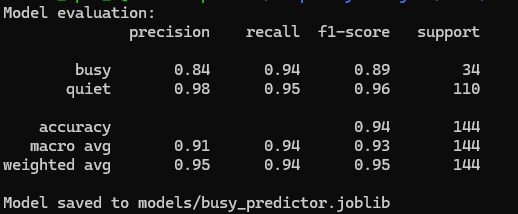
\includegraphics[width=0.8\textwidth]{ml_predictions.png}
		\caption{Εκπαίδευση και Αποτελέσματα Πρόβλεψης Μοντέλου Random Forest}
		\label{fig:ml_predictions}
	\end{figure}
	
	\section{Περιβάλλον Προσομοίωσης Αισθητήρων (Mock Sensors)}
	Για την ολοκληρωμένη δοκιμή του συστήματος κάτω από ποικίλες συνθήκες, αναπτύχθηκε ένα περιβάλλον προσομοίωσης αισθητήρων (\texttt{mocksensors.py}). Οι εικονικοί αισθητήρες λειτουργούν ανεξάρτητα από το φυσικό υλικό του Raspberry Pi και παράγουν συνεχώς συνθετικά δεδομένα τηλεμετρίας.
	
	Οι προσομοιωμένες μετρήσεις αφορούν το επίπεδο πληρότητας (απόσταση σε εκατοστά και ποσοστό \%), το βάρος των απορριμμάτων (kg), την εσωτερική θερμοκρασία (\textdegree C) και την κατάσταση της μπαταρίας (\%). Η χρήση των Mock Sensors επέτρεψε την ανάπτυξη και αποσφαλμάτωση του Node-RED, του REST API και του Home Assistant Dashboard χωρίς την ανάγκη διαρκούς φυσικής διέγερσης του συστήματος. Τα δεδομένα τους ακολουθούν την ίδια σημασιολογική δομή JSON-LD (SOSA) με τους πραγματικούς αισθητήρους.
	
	\section{Σχεδίαση UI και Dashboard μέσω Home Assistant}
	Παράλληλα με το βασικό dashboard που σχεδιάστηκε στην Python για τον έλεγχο και χρήση του έξυπνου κάδου, ενσωματώθηκε η open-source πλατφόρμα \textbf{Home Assistant} για την δημιουργία μιας διεπαφής όπου θα χρησιμοποιείται για την οπτικοποίηση στατιστικών, ιστορικού, αριθμό χρήσεων του συστήματός μας, και πολλά άλλα.
	
	\subsection{Περιγραφή Λειτουργιών}
	Το Dashboard διαθέτει έξι βασικές ενότητες λειτουργιών:
	
	\begin{itemize}
		
		\item \textbf{Markdown Card (System Diagnostics):} Εμφανίζει διάφορες πληροφορίες για το σύστημά μας, οι οποίες επιβεβαιώνουν την υγεία του (\texttt{Active\_Bins}, \texttt{Critical\_Alerts}, \texttt{Sensors}), καθώς και τον αριθμό χρήσεων την σημερινή μέρα και το πόσο γεμάτοι είναι οι κάδοι.
		\item \textbf{Bin Status Section (status, usage, motion counter):} Είναι ένα σύνολο καρτών, το οποίο αντιστοιχεί σε κάθε κάδο του συστήματός μας, όπου μας δίνει πληροφορίες σαν current status, usage level, motion counter, motion history, last recorded motion.
		\item \textbf{Sensor health section (status, MQTT message record, alert):}  Είναι ένα σύνολο καρτών, το οποίο αντιστοιχεί σε κάθε σένσορα του συστήματός μας, όπου μας δίνει πληροφορίες σαν online/offline status, dropped/published/retained MQTT messages, alert for sensor fail.
		\item \textbf{Mock Sensors Monitor (telemetry, testing, debugging):} Είναι ένα σύνολο καρτών το οποίο αντιστοιχεί στο περιβάλλον προσομοίωσης και δοκιμών του συστήματος, εμφανίζοντας σε πραγματικό χρόνο τις τιμές των εικονικών αισθητήρων τηλεμετρίας, όπως το fill percentage, το βάρος, την απόσταση από το καπάκι, τη θερμοκρασία και το ποσοστό μπαταρίας.
		\item \textbf{Edge AI Diagnostics Cards (current hour predictions, model telemetry):} Είναι ένα σύνολο καρτών, το οποίο αντιστοιχεί στον ML σένσορα του συστήματός μας, όπου μέσω του prediction model που έχουμε λαμβάνουμε την πρόβλεψη την χρήσης κάθε κάδου για την τρέχουσα ώρα και γραφήματα όπου μας δείχνουν το confidence level και το usage prediction για τις τελευταίες 12 ώρες.
		\item \textbf{Activity Intensity Overlay (actual usage counter):} Είναι η καταγραφή των πραγματικών χρήσεων κάθε κάδου, για τις τελευταίες 6 ώρες.
		\item \textbf{Fill Level Controls \& Alerts (capacity warnings, route dispatch):} Είναι η διαδραστική διεπαφή ελέγχου της πληρότητας των κάδων, η οποία εμφανίζει δυναμικά προειδοποιήσεις όταν η χωρητικότητα φτάσει σε οριακό επίπεδο, και επιτρέπει στον χειριστή την άμεση επιβεβαίωση ή την επίλυση των alerts .
	\end{itemize}
	
	\begin{figure}[H]
		\centering
		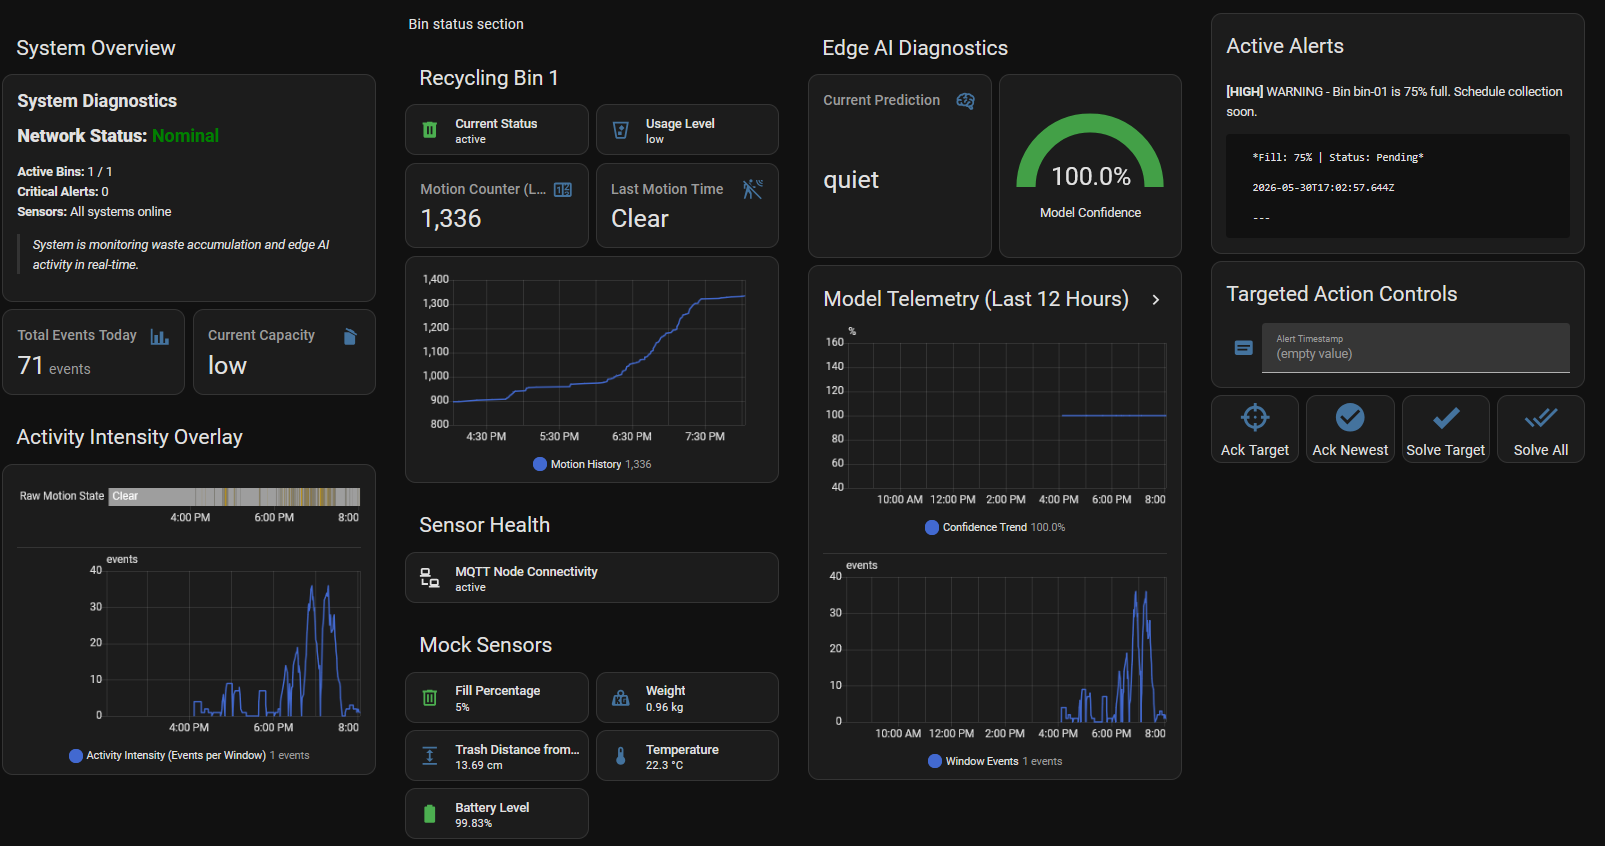
\includegraphics[width=0.9\textwidth]{Homeassistant.png}
		\caption{Διεπαφή Χρήστη (Dashboard) στο Home Assistant}
		\label{fig:home_assistant_dashboard}
	\end{figure}

	\section{Low-Code Ενορχήστρωση μέσω Node-RED}
	Παράλληλα με το UI του Home Assistant, ενσωματώθηκε η low-code πλατφόρμα \textbf{Node-RED} για την παροχή μιας ευέλικτης στρώσης ενορχήστρωσης, διαχείρισης συμβάντων και οπτικοποίησης.
	
	\subsection{Περιγραφή Ροών και Λειτουργιών}
	Στο Node-RED σχεδιάστηκαν και υλοποιήθηκαν έξι εξειδικευμένες ροές (Flows A έως Ε):
	
	\begin{itemize}
		\item \textbf{Flow A (Raw Sensor Monitor):} Λαμβάνει τα \texttt{fill\_level}, \texttt{weight}, \texttt{motion} του κάδου και τροφοδοτεί τα όργανα του Dashboard.
		\item \textbf{Flow B (Usage Intensity Replication):} Υλοποιεί μια λογική ελέγχου έντασης με κυλιόμενο παράθυρο 5 λεπτών, κατηγοριοποιώντας τη χρήση σε \texttt{LOW}, \texttt{MEDIUM}, \texttt{HIGH} και \texttt{CRITICAL} βάσει του \texttt{fill\_level} του κάδου.
		\item \textbf{Flow C (Alert Engine):} Σε περίπτωση \texttt{CRITICAL} κατάστασης, ενεργοποιεί pop-up ειδοποιήσεις στο Dashboard του NodeRed και στέλνει κλήσεις Webhook προς εξωτερικές υπηρεσίες.
		\item \textbf{Flow D (Data Router \& Archiver):} Λαμβάνει όλα τα μηνύματα μέσω wildcard (\texttt{smartbin/\#}) και τα αποθηκεύει σε έναν in-memory \textbf{κυκλικό buffer (circular buffer)} των τελευταίων 100 γεγονότων, ο οποίος είναι προσπελάσιμος μέσω REST API.
		\item \textbf{Flow Ε (Operator Summary Dashboard):} Ένα πλήρες, σκοτεινού θέματος (Catppuccin theme) Operator Dashboard που εμφανίζει live gauges, μετρητές σφαλμάτων, ενεργές ειδοποιήσεις και το χρόνο συνεχούς λειτουργίας του συστήματος (Uptime).
	\end{itemize}
	
	\begin{figure}[H]
		\centering
		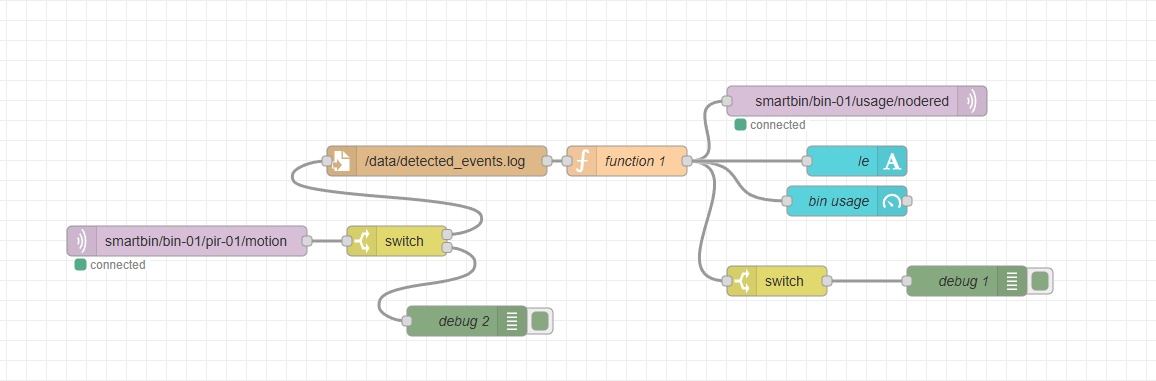
\includegraphics[width=0.95\textwidth]{nodered_flows.png}
		\caption{Υλοποίηση Ροών και Αυτοματισμών στο Node-RED}
		\label{fig:nodered_flows}
	\end{figure}
	
	\section{Μελλοντικές Επεκτάσεις (Future Implementation)}
	Το παρόν σύστημα σχεδιάστηκε με γνώμονα την επεκτασιμότητα, αφήνοντας περιθώριο για σημαντικές μελλοντικές βελτιώσεις:
	\begin{itemize}
		\item \textbf{Ενσωμάτωση Φυσικών Αισθητήρων:} Αντικατάσταση των σημερινών Mock Sensors με φυσικούς αισθητήρες υπερήχων (π.χ. HC-SR04), αισθητήρες βάρους (Load Cells) και θερμοκρασίας στο Raspberry Pi, για τη συλλογή πραγματικών δεδομένων.
		\item \textbf{Δημιουργία Βέλτιστων Δρομολογίων:} Χρησιμοποιούνται τα υπάρχων δεδομένα για υπολογισμό της βέλτιστης διαδρομής των απορριμματοφόρων, βάσει της πληρότητας και των προβλέψεων χρήσης.
		\item \textbf{Edge AI και Computer Vision:} Ενσωμάτωση καμερών και μοντέλων μηχανικής όρασης στον κάδο για την αναγνώριση του είδους των απορριμμάτων και την αυτόματη αξιολόγηση της σωστής χρήσης της ανακύκλωσης.
	\end{itemize}

	\section{Συμπεράσματα}
	Η υλοποίηση του συστήματος \textbf{Smart Waste Bin} απέδειξε την αξία του συνδυασμού παραδοσιακών γλωσσών προγραμματισμού (Python) με low-code εργαλεία (Node-RED) σε περιβάλλοντα IoT. Η χρήση του MQTT Broker ως κοινού διαύλου επικοινωνίας επέτρεψε την πλήρη αποσύνδεση (decoupling) των υπηρεσιών, καθιστώντας το σύστημα εξαιρετικά ανθεκτικό σε σφάλματα. 
	
	Η σημασιολογική μοντελοποίηση με JSON-LD προσφέρει τη δυνατότητα εύκολης ενσωμάτωσης των δεδομένων σε ευρύτερα οικοσυστήματα έξυπνων πόλεων, ενώ οι εικονικοί αισθητήρες κανόνων και μηχανικής μάθησης παρέχουν στους διαχειριστές πολύτιμη προγνωστική πληροφόρηση, επιτρέποντας τη βελτιστοποίηση των δρομολογίων αποκομιδής και τη μείωση του λειτουργικού κόστους.
	
	\section{Github Repository}
	Ο κώδικας του έργου βρίσκεται στο repository: \\
	\url{https://github.com/jimfil/smartWasteBinProject}.
	
	\begin{thebibliography}{99}
		\bibitem{sosa_ref} J. Compton et al., "The SSN ontology of the W3C semantic sensor network incubator group," \emph{Journal of Web Semantics}, 2012.
		\bibitem{mqtt_ref} A. Banks and R. Gupta, "MQTT Version 3.1.1," \emph{OASIS standard}, 2014.
		\bibitem{random_forest_ref} L. Breiman, "Random Forests," \emph{Machine Learning}, 2001.
	\end{thebibliography}
	
\end{document}